\documentclass{article}

\usepackage[utf8]{inputenc}
\usepackage{graphicx}
\usepackage{geometry}   \geometry{margin=1in}
\usepackage{amsmath}
\usepackage{xcolor}
\usepackage{float}
\usepackage{longtable}
\usepackage{natbib}
\usepackage[nonumberlist]{glossaries}

\makeglossaries
\loadglsentries{glossary}


\title{Hot Swappable Pedalboard and Routing System:\\Progress Report 2}
\author{Nicholas Pham}
\date{November 2018}

\begin{document}

\maketitle
\begin{center}
    Electrical Engineering \\
    Scott Kuindersma, Jim MacAurthur
\end{center}

\newpage
\glsaddall
\printglossaries
\newpage

\section{Define}
	\subsection{Introduction}
	\subsection{Motivation and Use Cases}
	\subsection{Background}
	\subsection{Specifications}
	The main issue with the current system of testing guitar pedals is the inconvenience and speed of switching between different units.  The following specifications directly relate to reducing the inconvenience and time required to swap between different units when demoing.

	\begin{center}
	\renewcommand{\arraystretch}{1.5}
	\begin{tabular}{|l|l|l|p{6cm}|}
		\hline
		Metric & Min Target Value & Preferred Target & Justification \\
		\hline
		Swapping Time & 80\% reduction & 90\% & To be useful, the solution should offer a major improvement in swap time.  As current swap time is on the order of 10 seconds, the improved switching time should be on the order of 1 second.\\
		Compatibility &  $>$80\% & $>$ 95\% & In order to be an effective tool, the solution must be usable with a majority of pedals available at typical retail locations.  80\% is reasonable because a majority of retailer stock contains pedals by a handful of brands.  There is a trade-off between compatibility versus function and form, so designing for any possible pedal is not possible. \\
		\hline
	\end{tabular}
	\end{center}

	After these primary specification follow several additional requirements which ensure that the solution will be useful.

	\begin{center}
	\renewcommand{\arraystretch}{1.5}
	\begin{longtable}{|l|l|l|p{7cm}|}
		\hline
		Metric & Min Target Value & Preferred Target & Justification \\
		\hline
		System Cost & \$200 & \$100 & Though the price of the solution when sold to a retailer is dependent on marketing and other factors, the cost to produce the system should be relatively low, so as to make it a viable option for use as a sales tool. \\
		Incremental Cost & \$20 & \$1 & There must also be a distinction drawn between the cost of an entire system and the cost of allowing an additional pedal to interface with the system.  Because many retail stores may stock hundreds of guitar pedals, the cost of adding a single new pedal to the system must be a small percent of that pedal's cost. \\
		Signal-to-Noise Ratio & 90dB &  120dB & The electric guitar, by virtue of its simple passive magnetic pickups can have a very high SNR, measured in non-ideal circumstances at +90 dBV.  Higher values in a controlled environment are likely.  Though many guitar pedals may have lower SNRs, it is vital the solution maintain the maximum possible dynamic range. \\
		Frequency Response & 20 - 20 kHz & DC - 30 kHz & As an audio system, the solution must at minimum pass the audio range.  Because the solution might be used with processors that could output DC voltages (such as control voltage signals), the frequency response should extend down to DC.  Ideally, the frequency response would exceed 20kHz to allow for higher frequency components generated by the guitar and nonlinear effects pedals. \\
		Switching Time & 125 ms & 20 ms & When swapping a pedal in or out of the system, there should be no perceptible delay between when the pedal is inserted and when the sound becomes effected.  125 ms is the threshold for detectability of sound latency against visuals \cite{BT1359-1}.  An ideal target would be in the range of tens of milliseconds, below which the Precedence effect suggests that there would be little discontinuity heard \cite{PrecedenceEffect}. \\
		Transient & $<$0.5 dB & $<$ 0.1 dB & When swapping a pedal in or out of the system, any transient created must not damage connected equipment (such as the amplifier) or be disturbing. \\
		SELV compliance	& Yes & - & For ease of design and safety, the solution should accept DC voltage from an external AC/DC converter.  Through Separated Extra Low Voltage (SELV) compliance, the solution will not need to design for high voltage safety, which would reduce design and regulation/testing costs. \\
		\hline
	\end{longtable}
	\end{center}

\section{Design}
	\subsection{System Level Description}
	- Describe approach \\
	- Include clear, well labeled diagrams of proposed solution \\
	- Discuss considerations and design choices \\
	\subsection{Design Choices}
		\subsubsection{Pedal-Plate Mounting}
		\subsubsection{Plate Material}
		\label{Plate Material}
		The design of the plates was mainly informed by the incremental cost specification.  To keep the cost of producing a single plate low, the plate should be as simple as possible to fabricate.  As the plate requires a relatively large surface area, at minimum the size of an "average" guitar pedal, yet does not require for function significant thickness, the ideal form would be a single sheet of material.  The important design considerations for the material are that 
		\begin{itemize}
			\item the material must be rigid on the scale of a 5 x 5 inch plate.
			\item the material must be thin enough for the screws of the bottom enclosure plates to easily pass through (less than)
			\item the material must be easily cut with readily available CNC tools, namely a laser cutter or router.
			\item the material must be inexpensive.
			\item the material must not be easily bent or broken by drops or bumps.
		\end{itemize}
		The initial prototypes for the pedal-plate mounting design used 1/8" acrylic, cut with a laser cutter, because it was easily accessible.  However, acrylic can be brittle \cite{}, so it is not a good choice for repeated handling by customers.  Another option was sheet aluminum, which has the benefit of being quite thin for its strength, making it easy for the pedal's screws to pass through.  A third option was to use the FR-4 grade glass epoxy resin used to make circuit boards.  In addition to being strong and lightweight, using this material allows for a simplification of the design.  Instead of sill needing to mount a circuit board to the main body of the plate, the circuit board can be the plate.  The physical layout of the screw slots can be cut at the same time as the board is shaped.  The wires to the plugs can escape directly from the surface of the board via a two position connector (such as the SWR201-NRTN-S02-SA-WH mated with a SWH201-NULN-S02-UU-WH from Sullins Connectors \cite{}). Other components such as switches used to select power can also be directly mounted and integrated with the board.  For its simplicity of design and manufacture, the first prototype will use this material and method for constructing the plates.

		\subsubsection{Plate-Receiver Electrical Connection Mechanism}
		Moving signal and power between the plate and receiver is a vital task.  Though a number of guitar pedals offer processing of stereo signals, most are fully monophonic, requiring only one input and output connection.  In addition, because almost every pedal uses a single supply (non-bipolar) voltage, the simplest scheme for connecting a plate to its receiver requires only four connections: Power, Ground, Input (Send), and Output (Return).  This means that it is feasible to transfer the signal directly with individual physical connections, rather than some serial data protocol such as $\text{I}^2\text{s}$, which might be used if there were many inputs and outputs.  The use of "hard-wire" connections also keeps the signal "pure" by eliminating any unnecessary processing, which is an important consideration for marketing purposes.

		Making a consistent electric connection between the plate and receiver calls for some sort of spring loaded connector.  Unlike the connectors mentioned in Section \ref{Plate Material}, these connections are easy to break if desired, but still maintain good contact when connected.  They do not require the two surfaces to be exactly aligned, and they require only the single part to operate (instead of a matching male and female connector).  Figure \ref{springloaded} shows some examples of spring loaded connectors.  On the left are connectors typically used to connect boards together within a product.  This class of spring connector is good for high pin count connections because of the large number of pins in a single unit, which are easy to manufacture cheaply.  For example, the 00-9258 type connector from AVX Corp costs \$0.77 for 8 electrodes from Digikey \cite{AVX_00-9258_Digikey}.  However, because these connectors are usually made for one time use when permanently assembling a product, they are not designed for repeated use.  For instance, the 00-9258 part is has a lifespan of just 50 cycles according to its datasheet \cite{AVX_00-9258_Datasheet}, which is certainly insufficient for this application.  For an order of magnitude estimate, each plate needs to be able to withstand 100 cycles per day for at least 1000 days (though the cycles/day is likely lower and the total days is likely higher).  This gives a ballpark estimate of 100,000 cycles minimum.

		\begin{figure}
			\begin{subfigure}{0.4\textwidth}
				\centering
				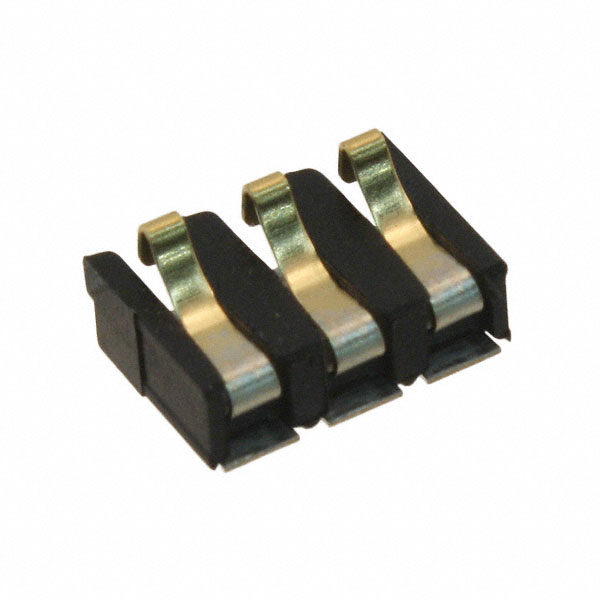
\includegraphics[width = 0.4\linewidth]{batteryconn.jpg}
			\end{subfigure}
			\begin{subfigure}{0.4\textwidth}
				\centering
				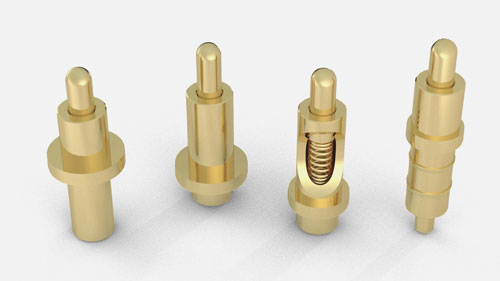
\includegraphics[width = 0.4\linewidth]{springpin.jpg}
			\end{subfigure}
			\label{fig:springloaded}
			\caption{Spring Loaded Connectors}
		\end{figure}

		In addition, because these connectors are designed for one time use, the order of connection does not matter.  However, for this application, there are some connections that must be "make-last, break-first," as will be described later.  This requires pins of different heights, which this type of multi-pin connector does not offer.  Instead, spring loaded pins like those on the right of Figure \ref{fig:springloaded} can be used.  This type of connector, sometimes known as a "Pogo Pin," includes a spring loaded plunger that sheaths into a sleeve.  These can be sourced through Digikey from Mill-Max, an industry standard manufacturer of milled connectors.  They have excellent electrical and mechanical characteristics, including 20m$\Omega$ contact resistance, minimum of 2 amp current rating, and a 1,000,000 cycle lifespan.  They come in a variety of lengths, though with less varied maximum strokes \cite{MillMax_025}.

		Using different length pins for different electrical connections allows some of these connections to be made or broken first.  In this case, most of the pins including signal and power will be of a standard height, but a shorter pin will be used to "mate-last, break-first" and will be used to ensure that the aforementioned connections are properly made before sending signal through to the plate.  In addition, a longer "mate-first, break-last" pin will be used as an inrush current limiter, as described in \cite{DesignforHotSwap}.

		Because these different pin heights are required, the design requires at least one of these spring loaded pins.  Their downside is in cost, as a pin like the costs about \$0.66 per pin.  Though the cost could be limited by using one of the multi-pin style connectors with a higher lifetime such as the Bourns 70AA series \cite{Bourns70AA_datahseet}, mixing the connection styles of the vertical-type spring loaded pins and the bending type multi-pin connectors would be difficult, in particular because of the difference in working heights.  The 0914 series spring loaded pins with the longest stroke length (for maximum height difference) are about 0.30" in height (before compression), while the uncompressed 70AA connector is 0.15" in height.  To mix these two types would require standoffs to adjust the uncompressed height, which determines the mate-order of the pins.  For simplicity, this prototype will use only pins from the 0914 series.

		Mill-Max offers many styles of spring loaded pins.  The first consideration was durability.  Though all of the pins examined are rated for 1,000,000 cycles \cite{MillMax_023}\cite{MillMax_025}, the through-hole versions likely offer better mechanical connection and stability with the circuit board, so these were preferred.  The next consideration was the ability to perform the mate-last, break-first operation, which requires as large a height differential as possible.  A large height differential will increase the time between the first and last pins making the connection, ensuring that the connections have been properly made and giving the circuit time to reach a steady state.  The pins are offered in short, standard, and long stroke lengths, which have maximum stroke depths of 0.039", 0.055", and 0.090" respectively. To achieve the longest time difference, the long stroke pins, series 0914 seem ideal.

		\begin{figure}
			\centering
			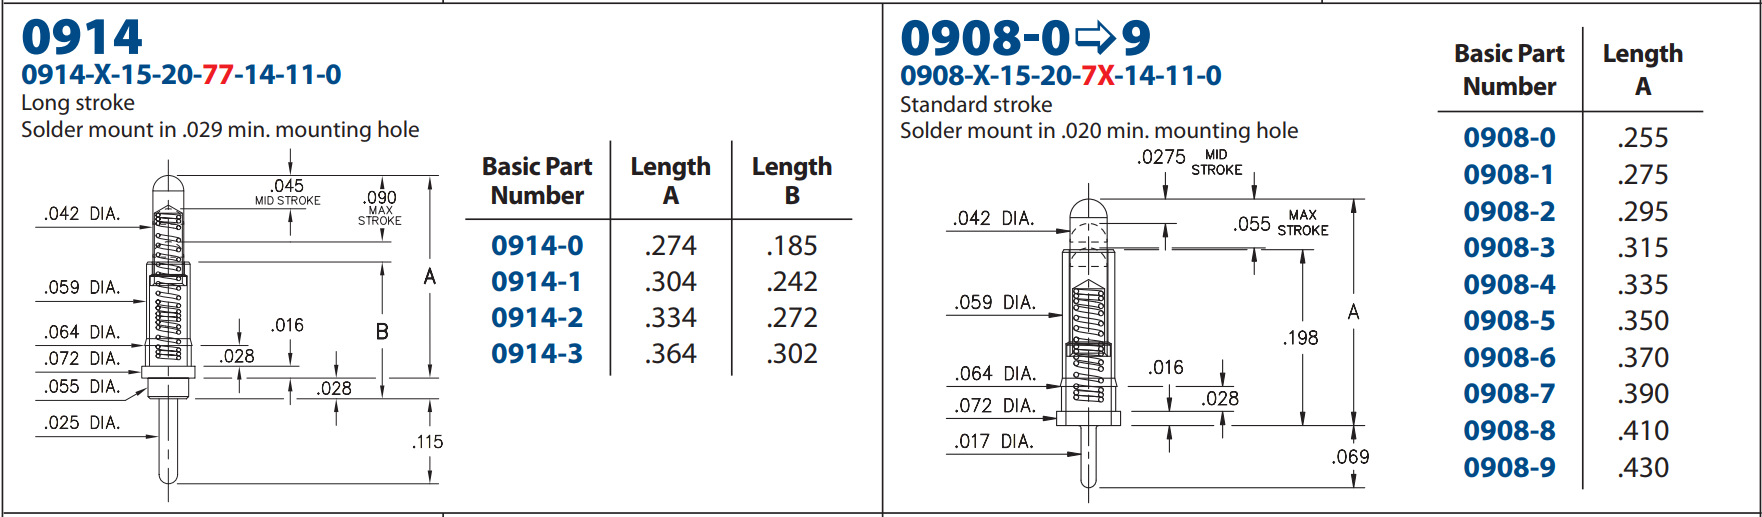
\includegraphics[width = \textwidth]{MillMaxSeries0914_0908.png}
			\caption{Mill Max Spring Pins, Through Hole, Long and Short Stroke}
			\label{fig:millmax0914_0908}
		\end{figure}

		As can be seen on the left in Figure \ref{fig:millmax0914_0908}, the B distance of the tallest pin determines the maximum travel of all of the pins, as this is the closest the plate can be to the surface of the receiver circuit board.  This means that 0914-0 and 0914-3 cannot be used together, as $B_3 = 0.302 == A_0 + 0.028 = 0.302$.  Only at 0914-3's maximum compression would 0914-0 make contact, so this will not work once the $\pm 0.006$ tolerances are taken into account.  However, any three consecutive pins will work together, which means choosing between using the 0914-0 and the 0914-3 (0914-1 and 0914-2 will be used in either case).  It turns out that the differences in length A any adjacent pins is 0.030", so the functional height difference between these two sets ({0, 1, 2} and {1, 2, 3}) are the same.  To reduce horizontal stress on the mounting, the shorter of the two options was chosen, as any tangential force on the end of the pin will result in less torque at the solder mount.  Thus the 0914-0 will be used for the make-last break first pins, the 0914-1 will be used for the standard input, output, and power pins, and the 0914-2 will be used for the inrush current limiting pin.

		\subsubsection{Plate Power Selection Method}
		In order to maximize the compatibility metric, the solution should be able to supply the most commonly required voltage and current supplies.  Though 9VDC is the de facto standard voltage supply \cite{pedallsit}, there are a number of effects that accept 12 or 18 VDC, which can allow their amplifiers to have a higher headroom.  There are some other less common power supplies, such as 24 VDC for some older Electro Harmonix products, or 9 VAC for pedals like the Line 6 DL4 \cite{Line6DL4manual}, but these are rarer, so this prototype will focus on just the 9, 12, and 18 VDC supplies.

		In addition to varying electrical requirements, some pedals do not use the standard 2.1 mm power jack, with the center connector wired negative; a common alternative is a 2.5 mm jack with center positive connection.  Though this first prototype will focus on providing just the standard 2.1 mm center negative power, an extension to alternative connectors can be easily added via additional power supply cables which can plug into the plate via the same SWH201-NULN-S02-UU-WH type connector mentioned in Section \ref{Plate Material}.

		In order to supply power to the plate, there were two schemes to consider.  The first was a parallel supply, where all three voltages are connected to the plate at once, and the user who sets up the plate for a particular pedal can choose which connector to attach the power connector to.  This would allow a single voltage regulator for each supply voltage to be used.  However, this could run into issues of current draw, where many pedals could potentially draw more current than the voltage regulator can handle.  In addition, this would mean long traces in the main board carrying this voltage, which might experience a voltage drop due to the resistance of these traces.  Finally, this scheme requires two pogo pins per available voltage, one for the make-first inrush current limiting and another for the normal power supply.  Figure \ref{fig:parallelpowerschematic} shows an implementation of such a scheme.


		The other option was to use a single voltage regulator for each plate, with a controllable output.  This eliminates concern over voltage drops between different receivers, and allows each receiver to draw as much current as a single regulator can supply.  For more than two power outputs, this method saves pogo pins, as only two pins are needed to supply the power (in addition to ground), though it does require several pins to communicate which voltage is desired for the current plate.  Instead of multiple connectors to allow the user to select the power connection, this method would use some switch, such as a two position DIP switch, to allow the user to set a binary value which can be decoded on the receiving end into the proper signals needed to control the adjustable voltage regulator.  As the pogo pins are fairly expensive (about \$0.66 each), reducing the number of pins is a good way to save on cost.

		The LM317 is a canonical adjustable voltage regulator, with its level set via a voltage divider (see datasheet section 8.2 for a typical application and design requirements \cite{LM317datasheet}).  The LM317 takes an input voltage between 1.25 and 37 V, preferably with $V_I - V_O > $ 3 V.  The difference $V_{OUT} - V_{ADJUST}$ is then kept at 1.25 V with a feedback circuit.  As shown in Figure \ref{fig:LM317_typicalapp}, this 1.25 V reference and $R_1$ then set the current through variable resistor $R_2$ ($I_{Adj}$ is negligible) which controls the output.  The $240 \Omega$ value for $R_1$ is a recommended value required to keep the output current high enough (over 3.5 mA) for a well regulated output.  The other diodes and capacitors are used to reduce ripple in the output.  Thus, $V_O$ can be given by

		\begin{align}
			V_O &= V_{REF}(1 + \frac{R_2}{R_1}) + I_{ADJ}R_2 \\
			&= 1.25 (1 + \frac{R_2}{240}) \quad \text{and} \\
			R_2 &= 240 \left( \frac{V_O}{1.25} - 1 \right) \\
			\label{eqn:LM317_R2}
		\end{align}

		However, a variable resistor for $R_2$ is not an easy method of setting the proper voltage for a user, because this would require individual tuning for each plate.  Instead, a set of switches is an easy mechanism for a user, who just needs to set the correct orientation of the switches.  A straightforward technique to use is switch in and out some additional resistors in parallel to a fixed $R_2$, as shown in Figure \ref{fig:adjustableregulatorschematic}.  Adding resistors in parallel reduces the effective resistance, reducing the output voltage, so the fixed $R_2$ should be calculated to set the maximum required output voltage, 18 VDC.  Using Equation \ref{eqn:LM317_R2} to calculate $R_2$ for an 18 V output gives $R_2 = 3.2 k\Omega$. The current through $R_1$ and consequently $R_2$ is $i_{R_1} = 1.25/240 = 5.2$ mA.  

		\begin{figure}
			\centering
			\includegraphics[width = 0.8\textwidth]{LM317_typapp}
			\caption{Typical Application of LM317, from datasheet.}
			\label{fig:LM317_typicalapp}
		\end{figure}

		\begin{figure}
			\centering
			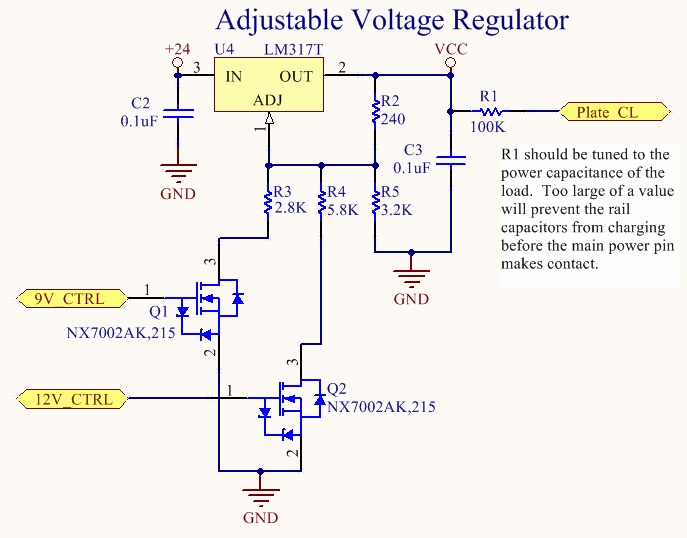
\includegraphics[width = 0.8\textwidth]{AdjustableRegulatorSchematic}
			\caption{MOSFET controlled adjustable regulator, with 9, 12, and 18 VDC selectable output.}
			\label{fig:adjustableregulatorschematic}
		\end{figure}

		MOSFETs are a good choice for this switch application because of their relatively low on-resistance $R_{DSon}$.  The cheapest type of MOSFET available from Digikey was the NX7002AK type, a ubiquitous single N-channel device \cite{NX7002AKdatasheet}.  With a maximum $V_{DS}$ of 60 V, a maximum $I_D$ of 190 mA for $V_{GS} = 10$ V at $25^o$ C, and a typical $R_{DSon}$ of $3.7 \Omega$ at $V_{GS}$ = 5V, this will work fine for this application, as would many standard MOSFETs.  In fact, because $R_{DSon}$ is on the order of Ohms while $R_2$ is on the order of Kiloohms, it can be neglected in the calculations for $R_3$ and $R_4$.

		For simplicity, let assume the MOSFET gate signals will not be turned on together, and that Q3 is used for a 9 V output while Q4 is used for a 12 V output, as in the following truth table:

		\begin{center}
		\begin{tabular}{c c|c}
			Q3 & Q4 & Output Voltage (V) \\
			\hline
			0 & 0 & 18 \\
			0 & 1 & 12 \\
			1 & 0 & 9 \\
			1 & 1 & X
		\end{tabular}
		\end{center}

		Because the MOSFET's on resistance can be ignored, solving for the $R_3$ when $Q_3$ is turned on so $R_3$ and $R_2$ are connected in parallel to ground gives

		\begin{align}
			R_3 || R_2 &= R_1 \left( \frac{V_O}{1.25} - 1 \right) = 240 \left( \frac{9}{1.25} - 1 \right) = 1488 \\
			R_3 &= \frac{1}{\frac{1}{R_3 || R_2} - \frac{1}{R_2}} = \frac{1}{\frac{1}{1488} - \frac{1}{3200}} = 2.8 k\Omega
		\end{align}

		Likewise, 

		\begin{align}
			R_4 || R_2 &= R_1 \left( \frac{V_O}{1.25} - 1 \right) = 240 \left( \frac{12}{1.25} - 1 \right) = 2064 \\
			R_4 &= \frac{1}{\frac{1}{R_4 || R_2} - \frac{1}{R_2}} = \frac{1}{\frac{1}{2064} - \frac{1}{3200}} = 5.8 k\Omega
		\end{align}

		Compute the power dissipated across these resistors to determine their necessary ratings.

		\begin{center}
		\begin{tabular}{c c|c}
			R ($k\Omega$) & V (V) & P (mW) \\
			\hline
			$R_1$ = 0.240 & 1.25 & 6.51 \\
			$R_2$ = 3.2 & 18 - 1.25 = 16.75 & 87.68 \\
			$R_3$ = 2.8 & 12 - 1.25 = 10.75 & 41.27 \\
			$R_4$ = 5.8 & 9 - 1.25 = 7.75 & 10.36
		\end{tabular}
		\end{center}

		Even with a 10\% safety margin, these resistors can all be 1/10 watt.



		\subsubsection{Receiver Plate-Removal Detection Method}
		\subsubsection{Receiver Bypass Mechanism}
		\subsubsection{Plate-Receiver Power Transfer}
		\subsubsection{Main Board Size}
		\subsubsection{Main Board Routing Options}
		\subsubsection{Main Board Routing Method}
		\subsubsection{Main Board Routing User Interface}
\section{Prototyping}
	- Explain chosen prototyping methods \\
	- Include CAD/schematic/flowchart/state diagrams of prototype \\
	- Reference components/data sheets, hardware, tools \\
\section{Measurements}
	In order to compare the performance of the prototype to the desired specifications, each metric must be measured.

	\subsection{Swapping Time}
	Measure the time required to swap one pedal for another.  As this is the simplest and most likely use scenario, and the swapping of a single pedal is the basis for all more complicated actions, this is a good metric for determining how much faster using the solution will be than the current method.  The experiment will start with a single pedal in series between the guitar and amplifier, with all necessary signal and power connections made.  The participant in the test plays the guitar through the pedal, validating that it the setup is functional.  On a signal, a timer starts while the guitarist stops playing, removes the current pedal from the signal chain, replaces it with the alternate pedal, which is readily on hand, and then tests that the new setup is functional by proceeding to play the guitar.  The timer stops once the participant begins playing again.

	It is important to use the same test procedure both when using the solution and when characterizing the typical method.  When testing the typical method, the guitarist must mute the amplifier to prevent popping, unplug signal and power from the pedal, plug in signal and power to the alternate pedal, then turn the amplifier on again.  When testing the solution system, the guitarist must lift the pedal plate out of the receiver, and insert the alternate pedal into the receiver.

	Because this test relies on a number of variables, including the person performing the test, it must be repeated multiple times per participant, with a number of different participants.  The participant should be told what steps need to be taken for a successful swap to be achieved in this test.

	\subsection{Compatibility}

	Using the list of all pedals available at a particular retail store, count the number of pedals on this list than will work with this solution electrically and mechanically.  In particular, for a pedal to be considered compatible, it must

	\begin{itemize}
		\item Be powered by a supply voltage and current available from the solution
		\item Use a power connector supported by the solution
		\item Be fully functional with the I/O available through the solution (single input and output)
		\item Have screw holes on the bottom plate that align for proper use with the plate mounting system
		\item Not be effected operationally by use of this solution
	\end{itemize} 

	If a pedal fits these criteria, it can be considered compatible with the solution.  The percentage of compatible pedals is the ratio of compatible pedals to the total number of pedals tested against these criteria.

	\subsection{Cost}

	In general, the cost should represent the cost for constructing a single unit of the solution, rather than price it would sell for, as the latter is too heavily affected by external factors.  However, the cost to produce a unit can be estimated by the sum of the material costs plus the estimated labor cost.  This will of course scale with volume, so an estimated volume should be on the order of the number of guitar retail stores in the United States, about 500.

	\subsection{Signal to Noise Ratio}
	$SNR = 20 \log \big( \frac{A_{signal}}{A_{noise}} \big)$.  When testing the unit, measure signal with sinusoid signal at varying frequencies in desired range (DC, 20Hz, 200Hz, 2kHz, 20kHz), as well as pink noise.  If possible, measure the system in a number of 

	\subsection{Frequency Response}
	The frequency response can be measured with the FFT function of an oscilloscope.  Input a sine wave swept from DC to 100 kHz and compare the ratio of the output to the input.

	\subsection{Switching Speed}
	Using an oscilloscope, measure the time difference between the detection of plate insertion and the relay switch settling on the desired output.  To determine the beginning of this period, look at the connection of the mate-last break-first pogo pins used to detect if the plate has been inserted or is being removed.  Determining the end of this period requires looking at the output signal.  To get a visual on when the output changes, connect the input of the system (the guitar end) to ground, and use a "pedal" whose output is always a known voltage, for example 5V.  The output will show a transition from 0V to 5V at the output when the plate containing this "pedal" is inserted.

	\subsection{Transient}
	The transient on the output signal due to switching can be due to a number of causes.  First, there may be an instantaneous difference between the input/bypass signal and the effected signal returning from the pedal.  One example of this might be a pedal that inverts the signal.  In addition, many pedals use a single supply voltage and have their amplifiers biased to Vcc/2, the leakage current through the decoupling capacitors on the input and output can cause nonzero voltages on the output if pull down resistors are not used, again leading to an instantaneous change in voltage level \cite{JackOrman}.

	Because these transients will occur differently each time, this must be tested with a variety of effects and in many trials.  Because the transients will have a strong high frequency component that will be very distinct from the typical signal, it should be easiest to detect them in the frequency domain.  To standardize the test and ease measurements, use a 1 kHz sine input and measure the power of any transients in the frequency domain, and compare to the standard power of the sine wave.  Perform with different pedals at different frequencies (100 Hz, 1 kHz, 10 kHz).

	\subsection{SELV Compliance}
	This should be evident from the design.  However, one test might be to verify that all signals in the device are below 60 VDC, which can be performed with a multimeter.

	
	- Describe planned measurements \\
		- Quantity to be measured \\
		- Methods and tools needed to perform measurement \\
	- "Student has appropriately implemented a technically rigorous mathematical model to address the design specifications"
\section{Analysis}
	- Describe how to compare measurements of system/subsystem performance against defined specs \\
	- Identify technically appropriate statistical methods for this analysis \\
	- Show thought towards visualization of the results \\
	- Discus how to use analysis to identify causes of discrepancies between actual and desired performance
\section{Logistics}
	- Project Time-line \\
	- Budget \\
	- Demonstrate Trainings and Approvals

\newpage
% \bibliographystyle{plain}
% \bibliography{ThesisSources}


\end{document}
